%%%%%%%%%%%%%%%%%%%%%%%%%%%%%%%%%%%%%%%%%%%%%%%%%%%%%%%%%%%%%%%%%%%%%%%%%%%%%%%%
%2345678901234567890123456789012345678901234567890123456789012345678901234567890
%        1         2         3         4         5         6         7         8

\documentclass[letterpaper, 10 pt, conference]{IEEEtran}  %
%\documentclass[letterpaper, 10 pt, conference]{ieeeconf}  %Comment this line out
                                                          % if you need a4paper
%\documentclass[a4paper, 10pt, conference]{ieeeconf}      % Use this line for a4
                                                          % paper

\IEEEoverridecommandlockouts                              % This command is only
                                                          % needed if you want to
                                                          % use the \thanks command
%%%%%%%%%%%%%\overrideIEEEmargins
% See the \addtolength command later in the file to balance the column lengths
% on the last page of the document



% The following packages can be found on http:\\www.ctan.org
%\usepackage{graphics} % for pdf, bitmapped graphics files
%\usepackage{epsfig} % for postscript graphics files
%\usepackage{mathptmx} % assumes new font selection scheme installed
%\usepackage{times} % assumes new font selection scheme installed
%\usepackage{amsmath} % assumes amsmath package installed
%\usepackage{amssymb}  % assumes amsmath package installed
\usepackage{cite}
\usepackage[utf8x]{inputenc}
\usepackage{amsmath,amssymb,amsfonts}
\usepackage{algorithm}
\usepackage[noend]{algorithmic}
\usepackage{graphicx}
\usepackage{textcomp}
\usepackage{multirow}
%\usepackage{hyperref}
% \usepackage{graphicx}
\title{\LARGE \bf
Analysis and Enhancement of the Simulated Binary Crossover*
}

%\author{ \parbox{3 in}{\centering Huibert Kwakernaak*
%         \thanks{*Use the $\backslash$thanks command to put information here}\\
%         Faculty of Electrical Engineering, Mathematics and Computer Science\\
%         University of Twente\\
%         7500 AE Enschede, The Netherlands\\
%         {\tt\small h.kwakernaak@autsubmit.com}}
%         \hspace*{ 0.5 in}
%         \parbox{3 in}{ \centering Pradeep Misra**
%         \thanks{**The footnote marks may be inserted manually}\\
%        Department of Electrical Engineering \\
%         Wright State University\\
%         Dayton, OH 45435, USA\\
%         {\tt\small pmisra@cs.wright.edu}}
%}

\author{\IEEEauthorblockN{Joel Chac\'on,
Carlos Segura}\\
\IEEEauthorblockA{Center for Research in Mathematics, Jalisco S/N, Col. Valenciana CP: 36023 Guanajuato, Gto, M\'exico}\\
\IEEEauthorblockA{joel.chacon@cimat.mx, carlos.segura@cimat.mx}% <-this % stops an unwanted space
}

% \author{Joel Chac\'on Castillo$^{1}$ and  Carlos Segura$^{2}$,
% \\{Center for Research in Mathematics, Jalisco S/N, Col. Valenciana CP: 36023 Guanajuato, Gto, M\'exico}\\
% {joel.chacon@cimat.mx, carlos.segura@cimat.mx}% <-this % stops an unwanted space
% % and Arturo Hen\'andez$^3$% <-this % stops a space
% %\thanks{*This work was not supported by any organization}% <-this % stops a space
% %\thanks{$^{1}$H. Kwakernaak is with Faculty of Electrical Engineering, Mathematics and Computer Science,
% %        University of Twente, 7500 AE Enschede, The Netherlands
% %        {\tt\small h.kwakernaak at papercept.net}}%
% %\thanks{$^{2}$P. Misra is with the Department of Electrical Engineering, Wright State University,
% %        Dayton, OH 45435, USA
% %        {\tt\small p.misra at ieee.org}}%
% }


\begin{document}



\maketitle
\thispagestyle{empty}
\pagestyle{empty}


%%%%%%%%%%%%%%%%%%%%%%%%%%%%%%%%%%%%%%%%%%%%%%%%%%%%%%%%%%%%%%%%%%%%%%%%%%%%%%%%
\begin{abstract}
Most recombination operators are designed to provide an adaptive behavior with the principle of altering its exploration capabilities depending on the diversity of the population.
%
However, depending only on the content of the population might be a drawback in long-term executions because diversity could not be large enough and the search process might prematurely converge.
%
Based on the previous scenario, a novel recombination operator is designed for tackling continuous Multi-objective Optimization Problems (MOPs), which works effectively to enhance the search capability of Multi-Objective Evolutionary Algorithms (MOEAs).
%
Particularly, this operator extends the Simulated Binary Crossover (SBX) by considering the stopping criterion to alter its internal operation.
%
In order to validate the effectiveness of our proposal, it is studied by substituting the original recombination operators in  three state-of-the-art MOEAs: NSGA-II, MOEA/D and SMS-EMOA.
%
The popular DTLZ, WFG and UF benchmark problems are taken into account.
%
Experimental validation shows a significant improvement in the performance of all the MOEAs when applying the novel crossover operator.
%
Additionally, our proposal are also tested against state-of-the-art differential evolution operators, providing quite competitive results.
%
\end{abstract}

\section{Introduction}
\label{Introduction}
Evolutionary Algorithms (EA) have become a promising alternative in several practical problems where is not suitable a deterministic approach.
%
Multi-objective Optimization Problems (MOPs) involves the simultaneous optimization of two or more objective functions that are usually in conflict.
%
A continuous minimization multi-objective problem can be defined as follows:
%
\begin{equation}\label{Base}
\begin{split}
&minimize \quad F(x) = (f_1(x), f_2(x), ..., f_m(x)) \\
&subject \quad to \quad x \in \Omega
\end{split}
\end{equation}
where $x = (x_1, ..., x_n) \in R^n$ indicate a decision variable vector, $n$ correspond to the number of decision variables, $\Omega$ is the feasible space, $F: \Omega \rightarrow R^m$ which consist of $m$ objective functions and $R^m$ is known as the \textit{objective space}.
%

Particularly, a MOP which consists in minimization of the $m$ objective functions and given two decision variable vectors $x, y \in \Omega$, $x$ dominates $y$ denoted by $x \prec y$, iff $f_i(x)  \leq f_i(y)$ for all objectives $\{1,...,m\}$, and the objective vectors are different $F(x) \neq F(y)$.
%
Accordingly this, the solution $x$ is not worse than $y$ in any of the objectives and $x$ is strictly better than $y$ in at least one objective.
%
The Pareto dominance is defined as the set of the best solutions that are not dominated by any feasible solution.
%
A decision variable vector $x^* \in \Omega$ is known as the Pareto optimal solution if does not exist any solution $x \in \Omega$ that dominates $x^*$.
%
The Pareto set correspond to the set of all Pareto optimal decision vectors and the Pareto front are the images of the Pareto set.
%
Principally, the goal in multi-objective optimization is to obtain an approximation of the Pareto front.
%
Therefore is required to obtain diverse and converged solutions among the Pareto front.
%

In the last decade several categories of Multi-Objective Evolutionary Algorithms (MOEAs) have been arising \cite{Joel:Kalyanmoy,Joel:Coello}, among them, the Non-Dominated Sorting Genetic Algortihm II (NSGA-II) \cite{Joel:NSGAII}, the MOEA based on decomposition (MOEA/D) \cite{Joel:MOEAD}, the $S$-metric Selection Evolutionary Multi-objective Optimization Algorithm (SMS-EMOA) \cite{Joel:SMSEMOA}, these representative methods are considered as ththat can bee state-of-the-art.


Differential Evolution (DE) is a popular algorithm and has showed a better performance than Genetic Algorithms (GAs) \cite{tuvsar2007differential, mi2010improved}.
%
However, it is well known that DE suffers of diversity issues, and presents a drawback in long-term executions.
%
This is because it has an aggressive convergence which can locate individuals in a sub-optimal region at the first stages of the execution, after that the rest of the function evaluations could be wasted.
%
To deal with this issues, the most recent algorithms are designed with strategies where is considered the criteria stop, such as adaptive parameters \cite{brest2017single}, Linear Population Size Reduction (LPSR) \cite{brest2008population} and several mutation strategies \cite{das2011differential}.
%
Also these adaptive strategies are oriented to deal with a substantial disadvantage, this is that are influenced by the crossover probability (CR) value and the mutation factor scale (F), therefore the quality of the solutions is highly affected by different configurations.
%
Also is evident the implications between single-objective and multi-objective problems which are related with the decision variable space diversity \cite{kukkonen2007performance}.

%
On the other hand GAs imply a less aggressive and flexible behavior, this can be a reason that DE performs to GAs in short-term executions both in continuous and discrete domains  \cite{tuvsar2007differential, mi2010improved}.
%
However, considering a long-term executions GAs have interesting properties, one of them is related with the probability density distribution that provides the flexibility of the operators that are involved, as the selection, crossover and  mutation operators.
%

In this paper, a novel recombination operator, is designed for tackling continuous multi-objective optimization problems (MOPs), which works effectively to enhance the search capability, guiding to a gradual change between exploration to intensification.
%
Therefore, several components of the Simulated Binary Crossover (SBX) are analyzed and modified, which aims to offer a suitable performance in long-term executions.
%

The rest of this paper is organized as follows.
%
In Section \ref{LiteratureReview} is provided a detailed review of the literature related with the SBX operator, and a brief description of the state-of-the-art of MOEAs.
%
Section \ref{Proposal} describes the key components of the SBX, and a dynamic behavior is imposed in each of these components, where an experimental analyzes is showed.
%
Therefore, our proposal is designed based in the effectively of each key component.
%
The experimental validation of the proposal and DE is showed in Section \ref{Experimental_Validation}.
%
Finally, conclusions and some lines of future work are given in Section \ref{Conclusions}.


\section{Literature Review}
\label{LiteratureReview}
This section is devoted to review some of the most important works that are highly related to the research presented in this paper.
%
Firstly, the most important MOEAs paradigms are defined.
%
Thereafter, some relevant classifications of crossover operators are discussed.
%
Finally, the popular Simulated Binary Crossover (SBX) operator is explained, which is used extensively in this paper.

\subsection{Multi-objective Evolutionary Algorithms}

Through the last years has been created a large number of MOEAs that follows different design principles.
%
In order to better classify them, several taxonomies have been proposed \cite{Joel:BOOK_MOEAs}.
%
Attending to the principles of design, MOEAs can be based on Pareto dominance, indicators and/or decomposition \cite{pilat2010evolutionary}.
%
Reciently, none of them have reported a clear advantage over the other ones.
%
Particularly, the experimental validation has been carried out by including the Non-Dominated Sorting Genetic Algorithm (NSGA-II) \cite{Joel:NSGAII}, the MOEA based on Decomposition \cite{Joel:MOEAD}, and the $S$-Metric Selection Evolutionary Multi-objective Optimization Algorithm (SMS-EMOA) \cite{Joel:SMSEMOA}.
%
Therefore, they are representative methods of the domination-based, decomposition-based and indicator-based paradigms, respectively.
%
The following subsections briefly describe each one of these paradigms, as well as the selected methods.

\subsubsection{Domination Based MOEAs - NSGA-II}

One of the most recognized paradigms are the domination based algorithms, particularly this family are based on the application of the dominance relation to design different components of the EAs.
%
Since that the dominance relation does not inherently promotes diversity in the objective space, auxiliary techniques such as niching crowding and/or clustering are usually integrated to obtain an acceptable spread and diversity in the objective space.
%
A critical drawback of the dominance relation is caused by the dimensionality of the objective space.
%
In fact the selection pressure is decremented substantially as the number of objectives increase.
%
Since this, some strategies have been developed to deal with this issue \cite{horoba2008benefits}.

%
One of the most popular techniques of this group is the NSGA-II.
%
This algorithm \cite{Joel:NSGAII} implements a special parent selection operator.
%
This operator is based on two mechanisms: fast-non-dominated-sort and crowding.
%
The first one tends to provide a convergence to the Pareto front and the second one promotes the preservation of diversity in the objective space.
%
A recent version is the NSGA-III, which is designed to deal with many-objective problems \cite{Joel:NSGAIII}.%  \cite{horoba2008benefits}.
%

\subsubsection{Decomposition Based MOEAs - MOEA/D}

Decomposition-based MOEAs \cite{Joel:MOEAD} transform a MOP in a set of single-objective optimization problems that are considered simultaneously.
%
This transformation can be achieved through several approaches.
%
The most popular of them is applying a weighted Tchebycheff function, therefore it is necessary provide weight vectors that are well distributed in the $m-1$ simplex that aims well-spread solutions.
%
However, an important drawback of this kind of approaches resides in the Pareto front geometry.
%
Particularly, the weight vectors could not be favorably to irregular Pareto front shapes.
%

MOEA/D \cite{Joel:MOEAD} is a recently designed decomposition-based MOEA.
%
It includes several principle such as problem decomposition, weighted aggregation of objectives and mating restrictions with neighborhoods definitions.
%
Particularly, the neighborhoods are considered in the variation operators.
%
A very used variant of the MOEA/D is the MOEA/D-DE, which use the DE operators \cite{price2006differential} and the polynomial mutation operator \cite{hamdan2012distribution} in the reproduction phase.
%
Additionally, it has two extra measures for maintaining the population diversity \cite{zhang2009performance}.
%
%However, these two extra mechanisms are not enough to deal with long-term executions.


\subsubsection{Indicator Based MOEAs - SMS-EMOA}

In multi-objective optimization several quality indicators have been developed to compare the performance of MOEAs.
%
Since these indicators measure the quality of the approximations attained by MOEAs, a paradigm based on the application of these indicators was proposed.
%
Particularly, instead of dominance concept, the indicators are used in the MOEAs to guide the optimization process.
%
Among the different indicators, hypervolume is a widely accepted Pareto-compliance quality indicator \cite{Joel:IGDPlus_And_GDPlus}.
%
The principal advantage of this algorithms is that the indicator usually takes into account both the quality and diversity of the solutions.
%

A popular and extensively used indicator-based algorithm is the SMS-EMOA \cite{Joel:SMSEMOA}.
%
This algorithm might be considered as hybrid, since it involves an indicator and dominance concepts.
%
Essentially, it integrates the non-dominated sorting method with the use of the hypervolume metric.
%
Thus, SMS-EMOA uses the hypervolume as a density estimator which results in a computationally extensive task.
%
Particularly, the replacement phase erases the individual of the worst ranked front with the minimum contribution to the hypervolume.
%
Taking into account the promising behavior of SMS-EMOA, it has been used in our experimental validation.
%
%
\begin{figure}[t]
\centering
\begin{tabular}{cc}
   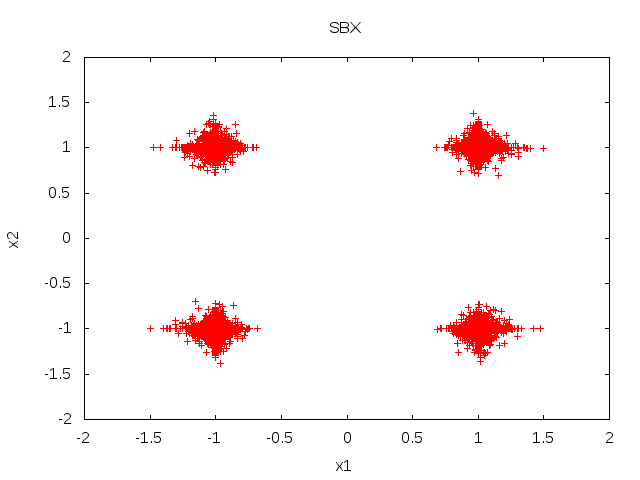
\includegraphics[width=0.25\textwidth]{img/SBX_eta_20_2D.png} 
   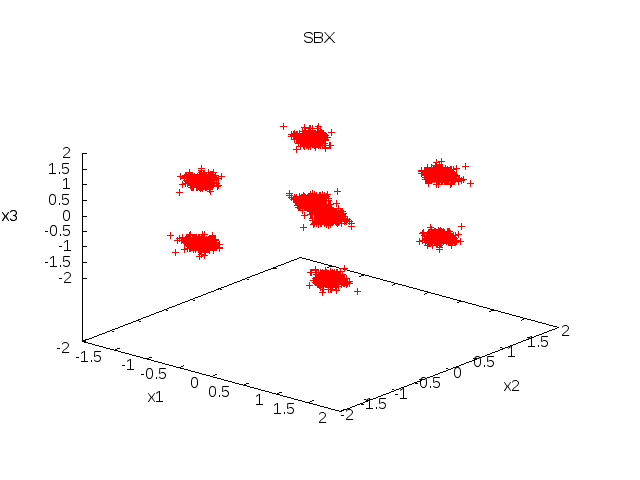
\includegraphics[width=0.25\textwidth]{img/SBX_eta_20_3D.png} 
\end{tabular}
\caption{Simulations of the SBX operator with a distribution index of 20, the parents are located in $P_1=(-1.0, -1.0)$ and $P_2=(1.0, 1.0)$ and $P_1=(-1.0, -1.0, -1.0)$ and $P_2=(1.0, 1.0, 1.0)$ for two and three variables respectively.}
\label{fig:Simulations_Index_20}
\end{figure}

\begin{figure}[!t]
\centering
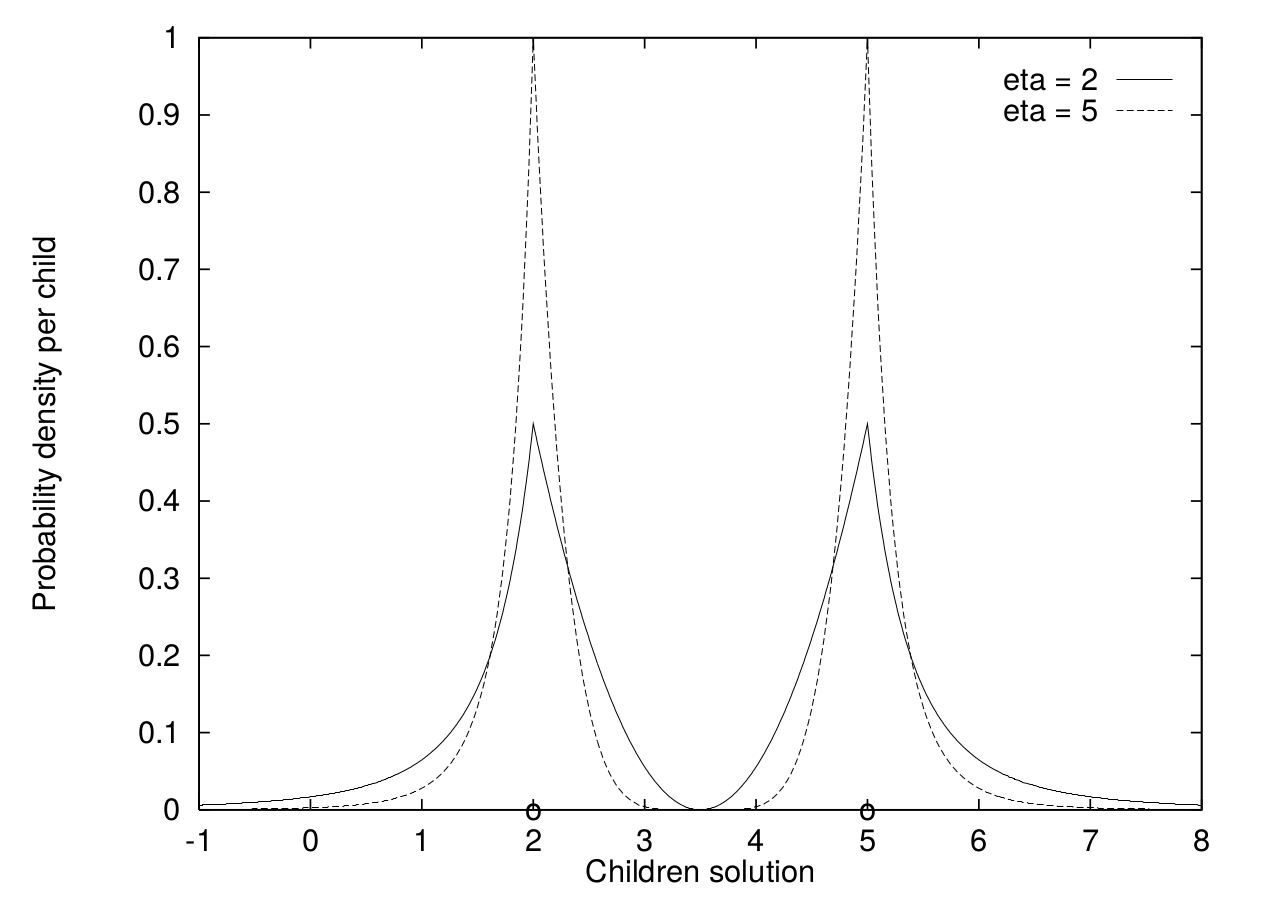
\includegraphics[width=2.5in]{img/DensitySBX_English.png}
\caption{Probability density function of the SBX operator with indexes of distribution 2 and 5. The parents are located in 2 and 5 respectively.}
\label{fig:fig_sim}
\end{figure}
\subsection{Crossover operators}
The crossover operators are designed to generate offspring solutions using information of the parent solutions.
%
They combine the feature of two or more parent solutions to form children solutions.
%
Since several crossover operators have been proposed, some taxonomies have also been provided.
%
The taxonomies are based on features such as the location of new generated solutions or the relation among the variables.
%

A popular taxonomy classifies crossover operators into variable-wise operators and vector-wise operators.
%
In the variable wise category, each variable from parent solutions is recombined independently with a certain pre-specified probability to create new values.
%
These operators are specially suitable to deal with separable problems.
%
Some operators belonging to this category are the Blend Crossover (BLX) \cite{eshelman1993real}, and the SBX \cite{Joel:SBX1994}.
%
On the other hand, the vector-wise recombination operators are designed to take into account the linkage among variables.
%
They usually perform a linear combination of the variable vectors.
%
Some operators belonging to this category are the Unimodal Normally Distributed Crossover (UNDX) \cite{Joel:UNDX}, and the simplex crossover (SPX) \cite{Joel:DE_Storn_SPX}.
%
Additionally, the crossover operators can be classified as Parent-Centric and Mean-Centric \cite{jain2011parent}.
%
In Parent-Centric operators, children solutions are created around one of the parent solutions, whereas in Mean-Centric operators, children solutions are created mostly around the mean of the participating parent solutions.
%
Among the crossover operators, SBX is probably the most frequently used operator, so this research focuses on this crossover.

\subsubsection{The Simulated Binary Crossover - SBX}

The reproduction operators are one of the most relevant components that influence the search process of the GAs.
%
Specifically, the crossover and mutation operators are highly related with the diversity of solutions.
%
Hence, the quality solutions can be affected.
%
%Particularly, in this paper is discussed the crossover operator.

The Simulated Binary Crossover (SBX) \cite{deb1994simulated} is popularly implemented in GAs \cite{Joel:NSGAII,Joel:SMSEMOA} and is classified as Parent-Centric, meaning that two children values ($c_1$ and $c_2$) are created around the parent values ($p_1$ and $p_2$).
%
Also the process of generate the children values is based in a probability distribution.
%
This distribution is defined by a non-dimensional variable, better known as the spread factor $\beta = |c_1 - c_2 | / |p_1 - p_2|$, indicating the ratio of the spread children values related with the parent values.
%

Additionally, this density function uses a distribution index $\eta_c$ (user-defined control parameter) that alters the exploration capability of the operator.
%
Specifically, a small index induces a larger probability of building children values more dissimilar than parents values, whereas with a high index are generated solutions more similar to the parents as is showed in the Figure \ref{fig:fig_sim}.
%

Principally, the SBX has non-zero probability of creating any number in the search space by recombining any two parent values from the search space.
%
The probability distribution to create an offspring value is defined as a function of a non-dimensionalized parameter $\beta \in [0, \infty]$ as follows:
%
\begin{equation}
    P(\beta)= 
\begin{cases}
     0.5(\eta_c + 1)\beta^{\eta_c},& \text{if} \quad \beta \leq 1\\
     0.5(\eta_c + 1) \frac{1}{\beta^{\eta_c + 2}} ,& \text{otherwise}
\end{cases}
\end{equation}
%
Based in the mean-preserving property of children values and parent values, the distribution probability has the following properties:
\begin{itemize}
\item Both offspring values are equi-distant from parent values.
\item There exist a non-zero probability to create offspring solutions in the entire feasible space from any two parent values.
\item The overall probability of creating a pair offspring values within the range of parent values is identical to the overall probability of creating two offspring values outside  the range of parent values.
\end{itemize}

\begin{figure}[t]
\centering
\begin{tabular}{cc}
   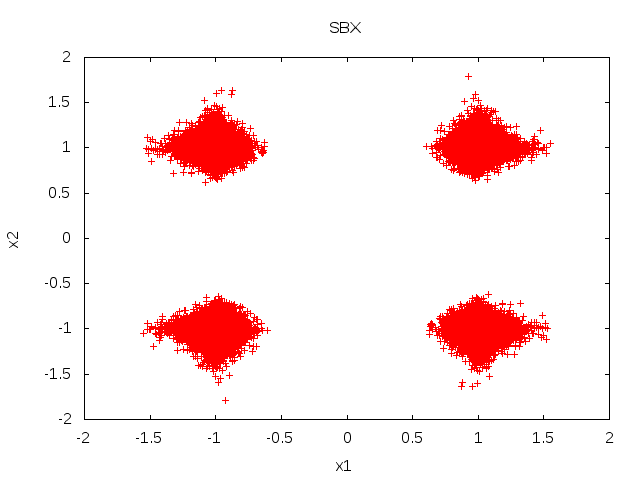
\includegraphics[width=0.25\textwidth]{img/SBX_eta_20_2D_pv_1.png} 
   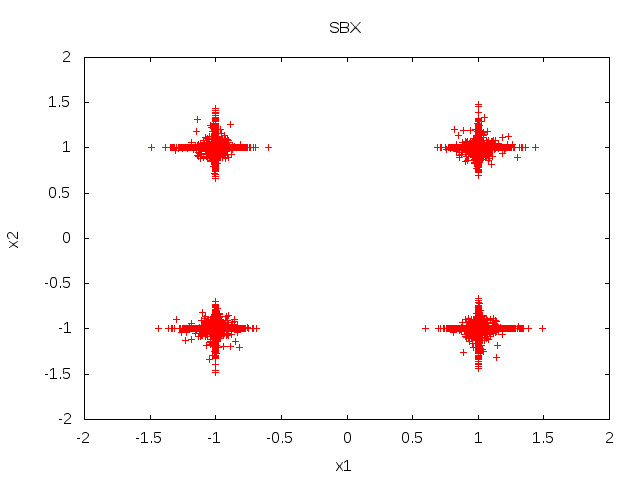
\includegraphics[width=0.25\textwidth]{img/SBX_eta_20_2D_pv_01.png} 
\end{tabular}
\caption{Simulations of the SBX operator with a distribution index of 20, the parents are located in $P_1=(-1.0, -1.0)$ and $P_2=(1.0, 1.0)$. The left simulation corresponds to a probability of altering a variable ($\delta_1$ in Algorithm \ref{alg:SBX_Operator}) to $1.0$ and in the right corresponds to $0.1$.}
\label{fig:Simulation_pv}
\end{figure}





Therefore, considering two participating parent values ($p_1$ and $p_2$), two offspring values ($c_1$ and $c_2$) can be created as linear combination of parent values with a random number $u \in [0, 1]$, as follows:
\begin{equation} 
\begin{split}
c_1 &= 0.5(1 + \beta(u))p_1 + 0.5(1 - \beta(u)) p_2 \\
c_2 &= 0.5(1 - \beta(u))p_1 + 0.5(1 + \beta(u)) p_2
\end{split}
\end{equation}

The parameter $\beta(u)$ depends on the random number $u$, as follows:
\begin{equation}
    \beta(u)= 
\begin{cases}
     (2u)^{\frac{1}{\eta_c+1}},& \text{if} \quad u \leq 0.5,\\
     	(\frac{1}{2(1-u)})^{\frac{1}{\eta_c +1}} ,& \text{otherwise}
\end{cases}
\end{equation}

The above equation only considers a optimization problem having no variable bounds.
%
In most practical problems, each variable is bounded within a lower and upper bound.
%
Thus, Deb and Beyer in 1999 \cite{deb1999self} proposed a modification of the probability distribution showed in the Equation (\ref{eq:sbx_spread}).
%
\begin{equation} \label{eq:sbx_spread}
    \beta(u)= 
\begin{cases}
     (2u(1-\gamma))^{\frac{1}{\eta_c+1}},& \text{if} \quad u \leq 0.5/(1-\gamma),\\
     	(\frac{1}{2(1-u(1-\gamma))})^{\frac{1}{\eta_c +1}} ,& \text{otherwise}
\end{cases}
\end{equation}
\begin{equation} \label{eq:child_1}
c_1 = 0.5(1 + \beta(u))p_1 + 0.5(1-\beta(u))p_2
\end{equation}
\begin{equation} \label{eq:child_2}
c_2 = 0.5(1 + \beta(u))p_1 + 0.5(1-\beta(u))p_2
\end{equation}
In this fashion, the child $c_1$ which is nearest to $p_1$ is calculated according the Equation (\ref{eq:child_1}).
%
Therefore, for $p_1 < p_2$ and the lower bound $a$ is closer to $p_1$ than to $p_2$, thus $\gamma = 1/(\alpha^{\eta_c + 1})$, where $\alpha = 1 + (p_1 - a) / (p_2 - p_1)$.
%
Similarly, the second child $c_2$ is computed with $\alpha = 1 + (b-p_2)/(p_2 - p_1)$, where $b$ correspond to the upper bound.
%
Then, the second child is computed as is indicated in the Equation (\ref{eq:child_2}).
\begin{algorithm}[t]
\algsetup{linenosize=\tiny}
\scriptsize
\caption{Simulated Binary Crossover (SBX)}
\label{alg:SBX_Operator}
\begin{algorithmic}[1]
    \STATE Input: Parents ($P_{1}, P_{2}$), Distribution index ($\eta_c$), Probability distribution ($P_c$).
    \STATE Output: Children ($C_{1}, C_{2}$).
    \IF{ $U[0, 1] \leq P_c$}
       \FOR{ each variable d}
	\IF{ $U[0, 1] \leq  \delta_1$} \label{alg:inherit_variable}
		\STATE Generate $C_{1,d}$ with Equations (\ref{eq:sbx_spread}) and (\ref{eq:child_1}).
		\STATE Generate $C_{2,d}$ with Equations (\ref{eq:sbx_spread}) and (\ref{eq:child_2}).
		 \IF{$ U[0, 1]  \geq  \delta_2 $} 
			\STATE Swap $C_{1,d}$ with $C_{2,d}$.
		 \ENDIF
        \ELSE
	   \STATE $C_{1,d} = P_{1, d}$.
	   \STATE $C_{2,d} = P_{2, d}$.
        \ENDIF
       \ENDFOR
    \ELSE
	\STATE $C_{1,d} = P_{1,d}$.
	\STATE $C_{2,d} = P_{2,d}$.
    \ENDIF
\end{algorithmic}
\end{algorithm}
In the literature \cite{Joel:SBX1994} is not entirely studied the SBX extension to multi-variables problems, in fact the authors implemented a similar mechanism to the uniform crossover for multiple variables \cite{Joel:UNDX} for choosing which variables to cross.
%
However those authors recognized the important implications with the linkage issues, therefore it does not alleviate the linkage problem of some MOPs.
%

\subsubsection{Implementation and analyses of SBX operator}
This section discusses the principal characteristics of SBX operator.
%
Essentially, the behavior of this operator is directly affected by three key components.
%
Firstly, it applies a probability of altering each variable which is fixed to $0.5$, therefore in average the half of each parent is duplicate in each child.
%
If this probability value is increased, the children values are more dissimilar, since that in average are modified more variables.
%
An appropriate setting of this probability is related with the MOP, therefore a high probability value is better with objective functions that have high dependence level in the parameters.
%
The behavior of variating this probability can be noticed in the Figure \ref{fig:Simulation_pv}, where a low probability provokes a bias to the axis (right side), being a suitable aproach for separable problems.
%
On the other hand, a high probability (left side) could be better in non-separable problems.
%
Additionally, this probability value is related with the distribution index, in fact both components have a direct effect in the similarity between parents and children.
%
%Otherwise, a low probability value is suitable for objective functions that are separable \cite{ma2016multiobjective}, due that few decision variables are modified by the crossover operation.
%
\begin{figure}[t]
\centering
\begin{tabular}{c}
   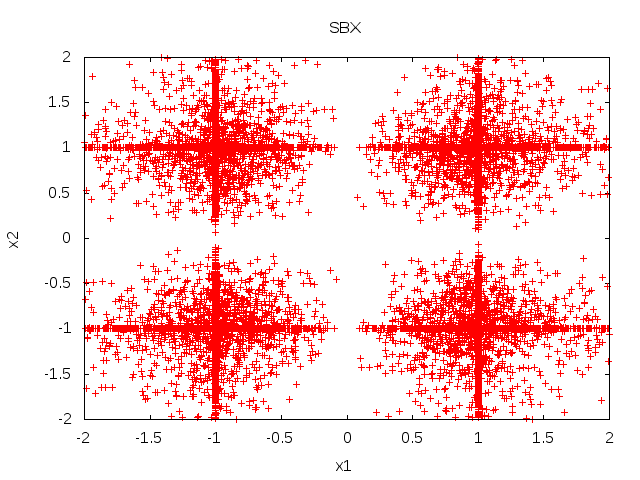
\includegraphics[width=0.24\textwidth]{img/SBX_eta_2.png}  %&
   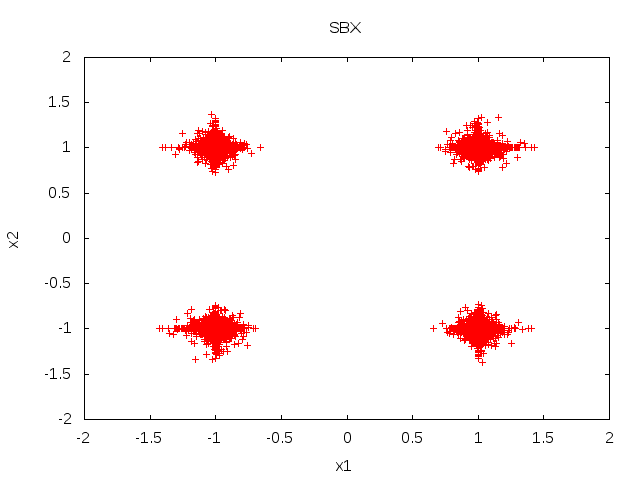
\includegraphics[width=0.24\textwidth]{img/SBX_eta_20.png} 
\end{tabular}
\caption{Simulation of the SBX operator sampling $10,000$ children values, the parents are located in $P_1=(-1.0, -1.0)$ and $P_2=(1.0, 1.0)$. The left and right are with a distribution index of $2$ and $20$ respectively.}
\label{fig:Simulation_Case_3}
\end{figure}
The second key component resides in that two child values are interchanged given a defined probability (usually $0.5$).
%
In some contexts this probability is known as ``Variable uniform crossover probability'' \cite{tuvsar2007differential} or ``Discrete Recombination'' \cite{muhlenbein1993predictive}.
%
Although that in single-objective this action provides an uto-adaptive behavior, in multi-objective optimization could not provide a desirable effect at first stages, the principal reason is that it could be highly disruptive.
%
This components has serial implications, since that interchange variables between the children has the effect of multiple ``reflections'' in the feasible space.
%
However, increasing the dimensions of the decision variables has the effect of increase exponentially the number of reflections ($2^{n}-2$) as is showed in the Figure \ref{fig:Simulations_Index_20} where are considered two and three decision variables.
%

Finally, the last component is the distribution index, which plays an important role, since a low index results in a greater exploration levels.
%
In fact a distribution index of the unity has the similar effect of the Fuzzy Recombination Operator \cite{voigt1995fuzzy}, the behaviour of the different indexes can be analyzed in the Figure \ref{fig:Simulation_Case_3} where in the left is showed a simulation which consider a low index value, whereas in the right is used a high index that create similar values of the parents.
%
Also can be noticed that it has a bias of create children according to the axis.
%

%
For simplicity the SBX implementation is showed in the Algorithm \ref{alg:SBX_Operator}, which is based in the most used implementation and is integrated in the NSGA-II code published by Deb et al. \cite{Joel:NSGAII}.
%
It requires two parents ($P_1$ and $P_2$) and create two children ($C_1$ and $C_2$).
%

Principally, the first and second key components correspond to the lines 5 and 8 respectively. 
%
As is usual, the SBX is configured with $\delta_1 = \delta_2 = 0.5$ and $\eta_c = 20$.
%
It is important take into account that this configuration neither considers the dimension of the decision variables space or the criteria stop.




% Please add the following required packages to your document preamble:
% \usepackage{multirow}
% \usepackage{graphicx}
\begin{table*}[t]
\centering

\caption{Statistical Information of Metrics with two objectives}
\label{tab:Metrics_2}
\resizebox{\textwidth}{!}{%
\begin{tabular}{|c|c|c|c|c|c|c|c|c|c|c|c|c|c|c|c|c|c|c|}
\hline
\multirow{2}{*}{} & \multicolumn{6}{c|}{NSGA-II} & \multicolumn{6}{c|}{MOEA/D} & \multicolumn{6}{c|}{SMS-EMOA} \\ \cline{2-19} 
 & 1 & 2 & 3 & 4 & 5 & DE & 1 & 2 & 3 & 4 & 5 & DE & 1 & 2 & 3 & 4 & 5 & DE \\ \hline
Average HV & 0.88 & 0.90 & 0.90 & 0.91 & 0.93 & \textbf{0.94} & 0.87 & 0.87 & 0.87 & 0.90 & \textbf{0.91} & \textbf{0.91} & 0.88 & 0.89 & 0.87 & 0.91 & 0.92 & \textbf{0.93} \\ \hline
Best Counts HV & 2 & 1 & 0 & 1 & 8 & \textbf{11} & 2 & 0 & 2 & 2 & 8 & \textbf{9} & 0 & 1 & 1 & 5 & 6 & \textbf{10} \\ \hline
\multicolumn{1}{|l|}{Average Best Difference HV} & \multicolumn{1}{l|}{0.068} & \multicolumn{1}{l|}{0.057} & \multicolumn{1}{l|}{0.053} & \multicolumn{1}{l|}{0.039} & \multicolumn{1}{l|}{0.019} & \multicolumn{1}{l|}{\textbf{0.017}} & \multicolumn{1}{l|}{0.053} & \multicolumn{1}{l|}{0.048} & \multicolumn{1}{l|}{0.049} & \multicolumn{1}{l|}{0.024} & \multicolumn{1}{l|}{\textbf{0.013}} & \multicolumn{1}{l|}{0.014} & \multicolumn{1}{l|}{0.074} & \multicolumn{1}{l|}{0.064} & \multicolumn{1}{l|}{0.081} & \multicolumn{1}{l|}{0.045} & \multicolumn{1}{l|}{0.028} & \multicolumn{1}{l|}{\textbf{0.019}} \\ \hline
Average IGD+ & 0.12 & 0.09 & 0.11 & 0.07 & 0.06 & \textbf{0.05} & 0.14 & 0.12 & 0.14 & 0.09 & 0.08 & \textbf{0.07} & 0.13 & 0.11 & 0.14 & 0.08 & 0.07 & \textbf{0.05} \\ \hline
Best Counts IGD+ & 2 & 1 & 1 & 1 & 8 & \textbf{10} & 3 & 0 & 2 & 3 & 6 & \textbf{9} & 0 & 2 & 0 & 3 & \textbf{9} & \textbf{9} \\ \hline
\multicolumn{1}{|l|}{Average Best Difference IGD+} & \multicolumn{1}{l|}{0.086} & \multicolumn{1}{l|}{0.052} & \multicolumn{1}{l|}{0.077} & \multicolumn{1}{l|}{0.035} & \multicolumn{1}{l|}{0.021} & \multicolumn{1}{l|}{\textbf{0.016}} & \multicolumn{1}{l|}{0.075} & \multicolumn{1}{l|}{0.059} & \multicolumn{1}{l|}{0.072} & \multicolumn{1}{l|}{0.025} & \multicolumn{1}{l|}{0.019} & \multicolumn{1}{l|}{\textbf{0.008}} & \multicolumn{1}{l|}{0.093} & \multicolumn{1}{l|}{0.071} & \multicolumn{1}{l|}{0.101} & \multicolumn{1}{l|}{0.038} & \multicolumn{1}{l|}{0.030} & \multicolumn{1}{l|}{\textbf{0.017}} \\ \hline
\end{tabular}%
}
\end{table*}

\section{Proposal}
\label{Proposal}
Based in the previous analysis, to achieve the effect of balance between exploration at first stages and intensification at the end of the executions the following modifications are proposed.
%
First, the probability of modify a variable ($P_v$) change among the execution, thus at first generations almost all variables are modified or sampled by the distribution and in the last stages less variables are sampled.
%
This change is based in a linear decrement model, where initially is 100\% and at the end it is 50\%.
%

In a similar way the second change is related with the ''variable uniform crossover probability`` which is incremented to the 50\%.
\begin{equation}
\delta = max \left (0.5, 1.0 - \frac{T_{Elapsed}}{T_{End}} \right )
\end{equation}

%
Finally, the index distribution change among the execution, where at the first stages it is low inducing a high degree of exploration and is incremented to the last stages as indicate the equation (\ref{eq:index_eta}).
\begin{equation}\label{eq:index_eta}
 \eta_c = 2 + 20 \times \left ( \frac{T_{Elapsed}}{T_{End}} \right)
\end{equation}


% Please add the following required packages to your document preamble:
% \usepackage{multirow}
% \usepackage{graphicx}
\begin{table*}[t]
\centering
\caption{Statistical Information of Metrics with three objectives}
\label{tab:Metrics_3}
\resizebox{\textwidth}{!}{%
\begin{tabular}{|c|c|c|c|c|c|c|c|c|c|c|c|c|c|c|c|c|c|c|}
\hline
\multirow{2}{*}{} & \multicolumn{6}{c|}{NSGA-II} & \multicolumn{6}{c|}{MOEA/D} & \multicolumn{6}{c|}{SMS-EMOA} \\ \cline{2-19} 
 & 1 & 2 & 3 & 4 & 5 & DE & 1 & 2 & 3 & 4 & 5 & DE & 1 & 2 & 3 & 4 & 5 & DE \\ \hline
Average HV & \textbf{0.87} & 0.84 & \textbf{0.87} & \textbf{0.87} & \textbf{0.87} & 0.85 & 0.84 & 0.84 & 0.84 & \textbf{0.86} & \textbf{0.86} & 0.85 & 0.90 & 0.89 & 0.88 & \textbf{0.91} & \textbf{0.91} & \textbf{0.91} \\ \hline
Best Counts HV & 1 & 2 & 1 & 4 & 4 & \textbf{7} & 1 & 2 & 1 & 2 & 5 & \textbf{8} & 3 & 2 & 0 & 2 & 5 & \textbf{7} \\ \hline
\multicolumn{1}{|l|}{Average Best Difference HV} & \multicolumn{1}{l|}{0.019} & \multicolumn{1}{l|}{0.047} & \multicolumn{1}{l|}{0.020} & \multicolumn{1}{l|}{\textbf{0.014}} & \multicolumn{1}{l|}{\textbf{0.014}} & \multicolumn{1}{l|}{0.032} & \multicolumn{1}{l|}{0.036} & \multicolumn{1}{l|}{0.041} & \multicolumn{1}{l|}{0.038} & \multicolumn{1}{l|}{0.016} & \multicolumn{1}{l|}{\textbf{0.013}} & \multicolumn{1}{l|}{0.027} & \multicolumn{1}{l|}{0.038} & \multicolumn{1}{l|}{0.038} & \multicolumn{1}{l|}{0.049} & \multicolumn{1}{l|}{\textbf{0.019}} & \multicolumn{1}{l|}{0.027} & \multicolumn{1}{l|}{\textbf{0.019}} \\ \hline
Average IGD+ & 0.13 & 0.16 & 0.13 & \textbf{0.12} & \textbf{0.12} & 0.13 & 0.15 & 0.14 & 0.15 & \textbf{0.11} & \textbf{0.11} & 0.13 & 0.11 & 0.11 & 0.13 & \textbf{0.09} & \textbf{0.09} & 0.13 \\ \hline
Best Counts IGD+ & 0 & 2 & 2 & 4 & 3 & \textbf{8} & 2 & 2 & 0 & 2 & 4 & \textbf{9} & 1 & 3 & 0 & 3 & 5 & \textbf{7} \\ \hline
\multicolumn{1}{|l|}{Average Best Difference IGD+} & \multicolumn{1}{l|}{0.029} & \multicolumn{1}{l|}{0.061} & \multicolumn{1}{l|}{0.027} & \multicolumn{1}{l|}{0.023} & \multicolumn{1}{l|}{\textbf{0.020}} & \multicolumn{1}{l|}{0.032} & \multicolumn{1}{l|}{0.053} & \multicolumn{1}{l|}{0.048} & \multicolumn{1}{l|}{0.053} & \multicolumn{1}{l|}{\textbf{0.015}} & \multicolumn{1}{l|}{\textbf{0.015}} & \multicolumn{1}{l|}{0.030} & \multicolumn{1}{l|}{0.047} & \multicolumn{1}{l|}{0.040} & \multicolumn{1}{l|}{0.062} & \multicolumn{1}{l|}{\textbf{0.020}} & \multicolumn{1}{l|}{0.024} & \multicolumn{1}{l|}{0.069} \\ \hline
\end{tabular}%
}
\end{table*}
\begin{table*}[t]
\centering
\caption{Summary of Statistical Tests}
\label{tab:statistical_Tests}
\begin{tabular}{|c|c|c|c|c|c|c|c|c|c|c|c|c|c|c|c|}
\hline
\multicolumn{16}{|c|}{NSGA-II} \\ \hline
 & \multicolumn{3}{c|}{1} & \multicolumn{3}{c|}{2} & \multicolumn{3}{c|}{3} & \multicolumn{3}{c|}{4} & \multicolumn{3}{c|}{5} \\ \hline
 & $\uparrow$ & $\downarrow$ & $\longleftrightarrow$ & $\uparrow$ & $\downarrow$ & $\longleftrightarrow$ & $\uparrow$ & $\downarrow$ & $\longleftrightarrow$ & $\uparrow$ & $\downarrow$ & $\longleftrightarrow$ & $\uparrow$ & $\downarrow$ & $\longleftrightarrow$ \\ \hline
\textbf{HV-2obj} & 16 & 29 & 47 & 6 & 61 & 25 & 28 & 19 & 45 & 31 & 23 & 38 & \textbf{54} & 3 & 35 \\ \hline
\textbf{HV-3obj} & 15 & 19 & 42 & 12 & 50 & 14 & 17 & 15 & 44 & \textbf{33} & 10 & 33 & 26 & 9 & 41 \\ \hline
\textbf{IGD-2obj} & 14 & 30 & 48 & 4 & 60 & 28 & 25 & 17 & 50 & 33 & 19 & 40 & \textbf{52} & 2 & 38 \\ \hline
\textbf{IGD-3obj} & 14 & 18 & 44 & 13 & 44 & 19 & 18 & 15 & 43 & \textbf{33} & 15 & 28 & 23 & 9 & 44 \\ \hline
% \end{tabular}
% \end{table*}

% \begin{table*}[]
% \centering
% \caption{My caption}
% \label{my-label}
% \begin{tabular}{|c|c|c|c|c|c|c|c|c|c|c|c|c|c|c|c|}
\hline
\hline
\multicolumn{16}{|c|}{MOEA/D} \\ \hline
 & \multicolumn{3}{c|}{1} & \multicolumn{3}{c|}{2} & \multicolumn{3}{c|}{3} & \multicolumn{3}{c|}{4} & \multicolumn{3}{c|}{5} \\ \hline
 & $\uparrow$ & $\downarrow$ & $\longleftrightarrow$ & $\uparrow$ & $\downarrow$ & $\longleftrightarrow$ & $\uparrow$ & $\downarrow$ & $\longleftrightarrow$ & $\uparrow$ & $\downarrow$ & $\longleftrightarrow$ & $\uparrow$ & $\downarrow$ & $\longleftrightarrow$ \\ \hline
\textbf{HV-2obj} & 15 & 33 & 44 & 10 & 60 & 22 & 25 & 26 & 41 & 39 & 18 & 35 & \textbf{57} & 9 & 26 \\ \hline
\textbf{HV-3obj} & 10 & 22 & 44 & 12 & 39 & 25 & 11 & 19 & 46 & 24 & 10 & 42 & \textbf{38} & 5 & 33 \\ \hline
\textbf{IGD-2obj} & 16 & 31 & 45 & 9 & 60 & 23 & 23 & 27 & 42 & 37 & 17 & 38 & \textbf{57} & 7 & 28 \\ \hline
\textbf{IGD-3obj} & 12 & 22 & 42 & 13 & 43 & 20 & 13 & 24 & 39 & 30 & 9 & 37 & \textbf{40} & 10 & 26 \\ \hline
% \end{tabular}
% \end{table*}

% \begin{table*}[]
% \centering
% \caption{My caption}
% \label{my-label}
% \begin{tabular}{|c|c|c|c|c|c|c|c|c|c|c|c|c|c|c|c|}
\hline
\hline
\multicolumn{16}{|c|}{SMS-EMOA} \\ \hline
 & \multicolumn{3}{c|}{1} & \multicolumn{3}{c|}{2} & \multicolumn{3}{c|}{3} & \multicolumn{3}{c|}{4} & \multicolumn{3}{c|}{5} \\ \hline
 & $\uparrow$ & $\downarrow$ & $\longleftrightarrow$ & $\uparrow$ & $\downarrow$ & $\longleftrightarrow$ & $\uparrow$ & $\downarrow$ & $\longleftrightarrow$ & $\uparrow$ & $\downarrow$ & $\longleftrightarrow$ & $\uparrow$ & $\downarrow$ & $\longleftrightarrow$ \\ \hline
\textbf{HV-2obj} & 9 & 35 & 48 & 7 & 43 & 42 & 16 & 31 & 45 & 41 & 9 & 42 & \textbf{53} & 8 & 31 \\ \hline
\textbf{HV-3obj} & 7 & 21 & 48 & 9 & 35 & 32 & 13 & 21 & 42 & 27 & 6 & 43 & \textbf{31} & 4 & 41 \\ \hline
\textbf{IGD-2obj} & 10 & 34 & 48 & 15 & 48 & 29 & 12 & 33 & 47 & 41 & 12 & 39 & \textbf{55} & 6 & 31 \\ \hline
\textbf{IGD-3obj} & 8 & 20 & 48 & 13 & 30 & 33 & 9 & 19 & 48 & 22 & 5 & 49 & \textbf{27} & 5 & 44 \\ \hline
\end{tabular}
\end{table*}

\section{Experimental validation}
\label{Experimental_Validation}
This section is devoted to validate our proposal (Case 5).
%
The WFG \cite{Joel:WFG}, DTLZ \cite{Joel:DTLZ_2} and UF \cite{zhang2009performance} test problems have been used for our purpose.
%
Our experimental validation includes the Differential Evolution based variants DEMO such strategy is explained in \cite{tuvsar2007differential}.
%
Given that all of them are stochastic algorithms, each execution was repeated $35$ times with different seeds.
%
The common configuration in all of them was the following: the stopping criterion was setted to $25,000$ generations, the population size was fixed to 100, the WFG test problems were configured with two and three objectives, setting 24 parameters, where 20 of them are distance parameters and 4 are position parameters.
%
Specifically, in the DTLZ test instances, the number of decision variables is set to $n=M+r-1$, where $r=\{5, 10, 20\}$ for DTLZ1, DTLZ2 to DTLZ6 and DTLZ7 respectively, as is suggested by the authors \cite{Joel:DTLZ_2}.  
% 
The UF benchmark is composed of ten test instances, where the first seven are of two objectives and the rest with three objectives, the number of decision variables is assigned to $n=10$.
%
In general, the crossover and mutation operators are SBX and polynomial respectively, with a crossover probability of 0.9 and mutation probability of $1/n$, also the crossover and mutation distribution indexes were assigned to 20 and 50 respectively.
%
The extra-parametrization of each algorithm is as follows:
\begin{itemize}
\item \textbf{DE-Variants}: CR = 0.3 and F = 0.5.
\item \textbf{SMS-EMOA}: offset = 100.
\item \textbf{MOEA/D}: size of neighborhood = 10, max updates by sub-problem (nr) = 2 and $\delta = 0.9$.
\end{itemize}
%
Our experimental analysis has been performed in base of the Normalized HV and IGD+.
%
The reference points implemented in the hypervolume indicator are showed in the Table \ref{tab:ReferencePoints} as used in \cite{Joel:Kuhn_Munkres, Joel:OperatorAHX}.


In order to statistically compare the hypervolume results, a similar guideline than the proposed in \cite{Joel:StatisticalTest} was used. 
%
First a Shapiro-Wilk test was performed to check whatever or not the values of the results followed a Gaussian distribution. 
%
If, so, the Levene test was used to check for the homogeneity of the variances. 
%
If samples had equal variance, an ANOVA test was done; if not, a Welch test was performed. 
%
For non-Gaussian distributions, the nonparametric Kruskal-Wallis test was used to test whether samples are drawn from the same distribution. 
%
An algorithm $X$ is said to win algorithm $Y$ when the differences between them are statistically significant, if the mean and median obtained by $X$ are higher than the mean and median achieved by $Y$.
%

In addition, pair-wise statistical tests with HV and IGD+ were performed (Table \ref{tab:statistical_Tests}).
%
For each instance, the column ``$\uparrow$'' reports the number of comparisons where the statistical tests confirmed the superiority of the MOEA listed in the corresponding group, whereas the column ``$\downarrow$'' reports the number of cases where it was inferior and ``$\longleftrightarrow$'' indicates that are not significantly different and are considered as a tie.
%%


Based in the statistical tests\footnote{DE is not considered in the statistical tests.} (Table \ref{tab:statistical_Tests}), generally speaking our proposal (Case 5) has the best scores.
%
Particularly, considering three objective and with the NSGA-II, the Case 4 is better than our proposal.
%
This might occurs for the ranking mechanism of this MOEA.
%
Since that the NSGA-II applies a binary tournament selection based in dominance concept and crowding procedure, thus an apropiate level of diversity is maintained.
%
As result some promising regions are reached.

%
Although that with three objective the Case 4 and our proposal have similar average results.
%
The average difference with the best indicates that our proposal is mostly closest to the best values.
%
This since that it shows $0.020$ in the ``Average Best Difference'' IGD+ against the Case 4 with $0.023$.
%
Also, inspecting the statistical tests, the Case 4 has more loses than our proposal ($10$ against $9$ and $15$ against $9$) of the HV and IGD+ respectively.
%
However, the MOEA/D and SMS-EMOA which are more elitist algorithms and do not consider the dominance concept at all, are not affected in this sense.
%
Anyway, our proposal and the Case 3 reports significantly better results that the normal SBX (Case 1), in fact this could evidence that variate the distribution index among the execution has an important effect.


In order to better understand the behavior of our proposal, the Tables \ref{tab:Metrics_2} and \ref{tab:Metrics_3} shows a summary average of Normalized HV and IGD+ considering all the instances\footnote{The detailed results can be consulted in the web page https:\//\//github.com\//joelchaconcastillo\//SBX\_CEC2018.}.
%
Also is counted the number of instances which attained the best results labeled by ``Best Counts''.
%
Additionally, the average of difference with the best result is showed, this aims to provide a metric which indicates the difference with the best result attained in each problem.
%

Although that the DE variants provides better average results than our proposal considering two objective, our proposal provides near solutions to the best, showing its stability.
%
Also according the number of objectives increase to three our proposal provides the best results.
%
The main reason is that DE is seriously deteriorated as the number of objectives increases, also it converges in a fast way, since it incorporates an agressive selection operator.
%

Despite the fact that DE variants have high ``Best Count'' values, in average it is improved by the Case 4 and Case 5, this might occurs because DE is directly influenced by the probability crossover ($CR$) and the mutation factor ($F$), therefore in some instances the DE variants attained the best results, and in other instances the solutions are far from the Pareto front.
%

On the other hand, our proposal shows a robust behavior in the state-of-the-art MOEAs, in fact the ``Average Best Difference'' is low both with two objectives and three objectives that confirms the stability and superiority of our proposal.
%
\begin{table}[t]
\centering
\scriptsize
\caption{References points for the HV indicator}
\label{tab:ReferencePoints}
\begin{tabular}{cc}
\hline
\textbf{Instances} & \textbf{Reference Point} \\ \hline
WFG1-WFG9 & $[2.1, ...,2m+0.1]$ \\
DTLZ 1, 2, 4 & $[1.1, ..., 1.1]$ \\
DTLZ 3, 5, 6 & $[3, ..., 3]$ \\
DTLZ7 & $[1.1, ..., 1.1, 2m]$ \\
UF 1-10 & $[2, ..., 2]$ \\ \hline
\end{tabular}
\end{table}
% % Please add the following required packages to your document preamble:
% % \usepackage{multirow}
% % \usepackage{graphicx}
% \begin{table*}[]
% \centering
% \caption{Statistical Information of Metrics}
% \label{my-label}
% \resizebox{\textwidth}{!}{%
% \begin{tabular}{|l|c|c|c|c|c|c|c|c|c|c|c|c|c|c|c|c|c|c|c|}
% \hline
% \multicolumn{2}{|l|}{\multirow{2}{*}{}} & \multicolumn{6}{c|}{NSGA-II} & \multicolumn{6}{c|}{MOEA/D} & \multicolumn{6}{c|}{SMS-EMOA} \\ \cline{3-20} 
% \multicolumn{2}{|l|}{} & 1 & 2 & 3 & 4 & 5 & 6 & 1 & 2 & 3 & 4 & 5 & 6 & 1 & 2 & 3 & 4 & 5 & 6 \\ \hline
% \multirow{6}{*}{2 Objectives} & Average HV & 0.88 & 0.90 & 0.90 & 0.91 & 0.93 & \textbf{0.94} & 0.87 & 0.87 & 0.87 & 0.90 & \textbf{0.91} & \textbf{0.91} & 0.88 & 0.89 & 0.87 & 0.91 & 0.92 & \textbf{0.93} \\ \cline{2-20} 
%  & Best Counts HV & 2 & 1 & 0 & 1 & 8 & \textbf{11} & 2 & 0 & 2 & 2 & 8 & \textbf{9} & 0 & 1 & 1 & 5 & 6 & \textbf{10} \\ \cline{2-20} 
%  & \multicolumn{1}{l|}{Average Best Difference HV} & \multicolumn{1}{l|}{0.068} & \multicolumn{1}{l|}{0.057} & \multicolumn{1}{l|}{0.053} & \multicolumn{1}{l|}{0.039} & \multicolumn{1}{l|}{0.019} & \multicolumn{1}{l|}{\textbf{0.017}} & \multicolumn{1}{l|}{0.053} & \multicolumn{1}{l|}{0.048} & \multicolumn{1}{l|}{0.049} & \multicolumn{1}{l|}{0.024} & \multicolumn{1}{l|}{\textbf{0.013}} & \multicolumn{1}{l|}{0.014} & \multicolumn{1}{l|}{0.074} & \multicolumn{1}{l|}{0.064} & \multicolumn{1}{l|}{0.081} & \multicolumn{1}{l|}{0.045} & \multicolumn{1}{l|}{0.028} & \multicolumn{1}{l|}{\textbf{0.019}} \\ \cline{2-20} 
%  & Average IGD+ & 0.12 & 0.09 & 0.11 & 0.07 & 0.06 & \textbf{0.05} & 0.14 & 0.12 & 0.14 & 0.09 & 0.08 & \textbf{0.07} & 0.13 & 0.11 & 0.14 & 0.08 & 0.07 & \textbf{0.05} \\ \cline{2-20} 
%  & Best Counts IGD+ & 2 & 1 & 1 & 1 & 8 & \textbf{10} & 3 & 0 & 2 & 3 & 6 & \textbf{9} & 0 & 2 & 0 & 3 & \textbf{9} & \textbf{9} \\ \cline{2-20} 
%  & \multicolumn{1}{l|}{Average Best Difference IGD+} & \multicolumn{1}{l|}{0.086} & \multicolumn{1}{l|}{0.052} & \multicolumn{1}{l|}{0.077} & \multicolumn{1}{l|}{0.035} & \multicolumn{1}{l|}{0.021} & \multicolumn{1}{l|}{\textbf{0.016}} & \multicolumn{1}{l|}{0.075} & \multicolumn{1}{l|}{0.059} & \multicolumn{1}{l|}{0.072} & \multicolumn{1}{l|}{0.025} & \multicolumn{1}{l|}{0.019} & \multicolumn{1}{l|}{\textbf{0.008}} & \multicolumn{1}{l|}{0.093} & \multicolumn{1}{l|}{0.071} & \multicolumn{1}{l|}{0.101} & \multicolumn{1}{l|}{0.038} & \multicolumn{1}{l|}{0.030} & \multicolumn{1}{l|}{\textbf{0.017}} \\ \hline
% \multirow{6}{*}{3 Objectives} & Average HV & \textbf{0.87} & 0.84 & \textbf{0.87} & \textbf{0.87} & \textbf{0.87} & 0.85 & 0.84 & 0.84 & 0.84 & \textbf{0.86} & \textbf{0.86} & 0.85 & 0.90 & 0.89 & 0.88 & \textbf{0.91} & \textbf{0.91} & \textbf{0.91} \\ \cline{2-20} 
%  & Best Counts HV & 1 & 2 & 1 & 4 & 4 & \textbf{7} & 1 & 2 & 1 & 2 & 5 & \textbf{8} & 3 & 2 & 0 & 2 & 5 & \textbf{7} \\ \cline{2-20} 
%  & \multicolumn{1}{l|}{Average Best Difference HV} & \multicolumn{1}{l|}{0.019} & \multicolumn{1}{l|}{0.047} & \multicolumn{1}{l|}{0.020} & \multicolumn{1}{l|}{\textbf{0.014}} & \multicolumn{1}{l|}{\textbf{0.014}} & \multicolumn{1}{l|}{0.032} & \multicolumn{1}{l|}{0.036} & \multicolumn{1}{l|}{0.041} & \multicolumn{1}{l|}{0.038} & \multicolumn{1}{l|}{0.016} & \multicolumn{1}{l|}{\textbf{0.013}} & \multicolumn{1}{l|}{0.027} & \multicolumn{1}{l|}{0.038} & \multicolumn{1}{l|}{0.038} & \multicolumn{1}{l|}{0.049} & \multicolumn{1}{l|}{\textbf{0.019}} & \multicolumn{1}{l|}{0.027} & \multicolumn{1}{l|}{\textbf{0.019}} \\ \cline{2-20} 
%  & Average IGD+ & 0.13 & 0.16 & 0.13 & \textbf{0.12} & \textbf{0.12} & 0.13 & 0.15 & 0.14 & 0.15 & \textbf{0.11} & \textbf{0.11} & 0.13 & 0.11 & 0.11 & 0.13 & \textbf{0.09} & \textbf{0.09} & 0.13 \\ \cline{2-20} 
%  & Best Counts IGD+ & 0 & 2 & 2 & 4 & 3 & \textbf{8} & 2 & 2 & 0 & 2 & 4 & \textbf{9} & 1 & 3 & 0 & 3 & 5 & \textbf{7} \\ \cline{2-20} 
%  & \multicolumn{1}{l|}{Average Best Difference IGD+} & \multicolumn{1}{l|}{0.029} & \multicolumn{1}{l|}{0.061} & \multicolumn{1}{l|}{0.027} & \multicolumn{1}{l|}{0.023} & \multicolumn{1}{l|}{\textbf{0.020}} & \multicolumn{1}{l|}{0.032} & \multicolumn{1}{l|}{0.053} & \multicolumn{1}{l|}{0.048} & \multicolumn{1}{l|}{0.053} & \multicolumn{1}{l|}{\textbf{0.015}} & \multicolumn{1}{l|}{\textbf{0.015}} & \multicolumn{1}{l|}{0.030} & \multicolumn{1}{l|}{0.047} & \multicolumn{1}{l|}{0.040} & \multicolumn{1}{l|}{0.062} & \multicolumn{1}{l|}{\textbf{0.020}} & \multicolumn{1}{l|}{0.024} & \multicolumn{1}{l|}{0.069} \\ \hline
% \end{tabular}%
% }
% \end{table*}


% \begin{figure}[!t]
% \centering
% \includegraphics[scale=0.25,angle=-90]{img/bar_HV_2obj.eps}
% \caption{Average of normalized hypervolume considering all the instances and two objective.}
% \label{fig_sim}
% \end{figure}
% \begin{figure}[]
% \centering
% \includegraphics[scale=0.25,angle=-90]{img/bar_IGD_2obj.eps}
% \caption{Average of Inverted Genralized Distance Plus (IGD+) considering all the instances and two objective.}
% \label{fig_sim}
% \end{figure}

% \begin{figure}[!t]
% \centering
% \includegraphics[scale=0.25,angle=-90]{img/bar_HV_3obj.eps}
% \caption{Average of normalized hypervolume considering all the instances and three objective.}
% \label{fig_sim}
% \end{figure}
% \begin{figure}[]
% \centering
% \includegraphics[scale=0.25,angle=-90]{img/bar_IGD_3obj.eps}
% \caption{Average of Inverted Genralized Distance Plus (IGD+) considering all the instances and three objective.}
% \label{fig_sim}
% \end{figure}






\section{Conclusions}
\label{Conclusions}

Crossover is one of the most important operators in EAs.
%
In most cases, crossover operators provide a large degree of exploration when the content of the population is diverse.
%
However, when a low diversity degree is reached, they tend to  promote intensification.
%
Since the behavior of operators does not usually depend on the stopping criterion, losing diversity in a gradual way might be a complex task.
%
Thus, some parameterizations might be suitable for some stopping criterion but not for others.
%
This paper proposes extending the well-known SBX to incorporate the stopping criterion and elapsed generations as one of its inputs.
%
First, the standard version of SBX and some actions that can be done to alter its exploration capabilities are identified.
%
Specifically, the SBX is composed by three key components that are related with diversity issues.
%
The first controls the amount of variables that are inherited intact.
%
The second is the probability of interchanging a given variable between offspring.
%
Finally, the last component is related with the aperture of the distribution index.
%
These tree features are adapted by taking into account both the stopping criterion and elapsed generations, with the aim of inducing an additional degree of exploration in the first stages of the optimization.
%
The experimental validation is carried out with long-term executions and the popular WFG, DTLZ and UF problems.
%
This validation shows that a dynamic distribution index provides significantly better and more robust results than the standard SBX with all the tested MOEAs.
%
Additionally, adapting the probability of interchanging variables between offspring provides benefits and by adapting this probability simultaneously with the distribution index performance can be further improved.
%
In the case of three objectives, state-of-the-art DE operators could also be outperformed by our proposal.
%
No additional parameterizations were required to devise the proposed operators, meaning that robust results could be obtained with the additional user efforts.
%An additional advantage is that does not required a distribution index a difference of the normal SBX.

Several lines of the future work might be explored.
%
First, we would like to devise some strategies to adaptively manage the distribution index.
%
Meassuring the diversity of the population to alter the behavior of the operators seems a plausible approach.
%
Additionally, using these kinds of operators together with some of the specific methods that has been devised to avoid premature convergence might bring additional benefits.
%
Finally, we plan to use the principles that governed the design of our proposals to devise novel vector-wise operators. 
%


%
%\addtolength{\textheight}{-12cm}   % This command serves to balance the column lengths
                                  % on the last page of the document manually. It shortens
                                  % the textheight of the last page by a suitable amount.
                                  % This command does not take effect until the next page
                                  % so it should come on the page before the last. Make
                                  % sure that you do not shorten the textheight too much.

%%%%%%%%%%%%%%%%%%%%%%%%%%%%%%%%%%%%%%%%%%%%%%%%%%%%%%%%%%%%%%%%%%%%%%%%%%%%%%%%



%%%%%%%%%%%%%%%%%%%%%%%%%%%%%%%%%%%%%%%%%%%%%%%%%%%%%%%%%%%%%%%%%%%%%%%%%%%%%%%%



%%%%%%%%%%%%%%%%%%%%%%%%%%%%%%%%%%%%%%%%%%%%%%%%%%%%%%%%%%%%%%%%%%%%%%%%%%%%%%%%
%\section*{APPENDIX}
%
%Appendixes should appear before the acknowledgment.
%
%\section*{ACKNOWLEDGMENT}
%
%The preferred spelling of the word ÒacknowledgmentÓ in America is without an ÒeÓ after the ÒgÓ. Avoid the stilted expression, ÒOne of us (R. B. G.) thanks . . .Ó  Instead, try ÒR. B. G. thanksÓ. Put sponsor acknowledgments in the unnumbered footnote on the first page.



%%%%%%%%%%%%%%%%%%%%%%%%%%%%%%%%%%%%%%%%%%%%%%%%%%%%%%%%%%%%%%%%%%%%%%%%%%%%%%%%
%
%References are important to the reader; therefore, each citation must be complete and correct. If at all possible, references should be commonly available publications.

\bibliographystyle{IEEEtran.bst}
% argument is your BibTeX string definitions and bibliography database(s)
\bibliography{IEEEabrv,example}

\end{document}
